\hypertarget{events}{%
\section{Events}\label{events}}

\begin{itemize}
    \item Interrupts are in the foregronud
    \item Events are in the background
\end{itemize}

\begin{figure}[H]
\centering
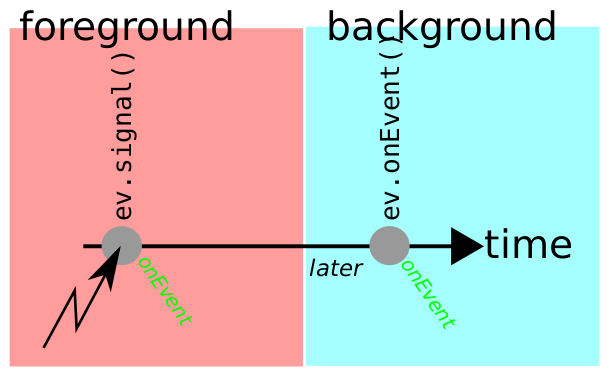
\includegraphics[width=0.6\textwidth]{figures/interruptsVsEvents.png}
\caption{Interrupts vs. Events}
\end{figure}

Im Interrupt selbst
sollten nur die dringenden Dinge behandelt werden. Alles andere, das
noch ein bisschen warten kann, soll auf später verschoben werden. In C++
wird dies mit Signals und Events gemacht. Im Interrupt wird ein Signal
gesetzt und später bei gegebener Zeit mit dem Eventhandler behandelt.

In unserem Beispiel von Events nennt sich der Background die Interrupts,
welche die Signale auslösen und in der Eventqueue abspeichern. Der
Foreground ist die Behandlung dieser Event-Queue.

\hypertarget{atomic}{%
\subsection{Atomic}\label{atomic}}

Damit beim signalisieren eines Events keine Race-Condition entsteht,
müssen die Events atomar signalisiert werden. Die Race-Condition kann
entstehen, wenn der eine Prozess versucht ein Event in die Queue zu
legen und von einem Interrupt unterbrochen wird, der sich ebenfalls an
der Queue zu schaffen macht.

\begin{verbatim}

\end{verbatim}

\begin{lstlisting}
void Event :: signal()
{
    __atomic_exchange_n(&queue.tail, this)->next=this;
}
\end{lstlisting}

\clearpage